\documentclass[10pt,conference,compsocconf]{IEEEtran}

%\usepackage{times}
%\usepackage{balance}
\usepackage{url}
\usepackage{graphicx}	% For figure environment
\usepackage{tikz}
\usepackage{pgfplots}
\usetikzlibrary{calc,intersections,through,backgrounds, shapes}
\newcommand{\rfig}[1]{Figure~\ref{fig:#1}}


\begin{document}
\title{CIL Project: Collaborative Filtering}

\author{
	Ulla Aeschbacher, David Eschbach,  Xiyue Shi, Fanyi Zhou\\
	Department of Computer Science, ETH Zurich, Switzerland
}

\maketitle

\begin{abstract}
Recommender systems and collaborative filtering have become very popular lately. For example streaming platforms use them to recommend new movies to their users based on ratings that users have previously assigned to other movies. For this purpose recommender systems try to exploit similarities between the rated items and potentially also between users. To achieve this, collaborative filtering aims to learn a low dimensional representation of those items.

In this paper we present our approach to the problem, which is based on a combination of Singular Value Decomposition (SVD) and k-nearest-neighbors (KNN) working with the Pearson correlation. Our final solution has a Root Mean Square Error (RMSE) of 0.98362.
\end{abstract}

\section{Introduction}
Collaborative filtering has been known for a while and there are many important contributions by research. For example in \cite{breese} there is an overview and an empirical analysis of multiple algorithms including memory-based algorithms predicting the rating of an item by the active user based on a weighted sum of the other users' rating of that item. Another example taken from \cite{breese} are model-based algorithms like the Bayesian Network Model that take a probabilistic approach to the problem by setting the rating to its expected value according to some probability distribution. In \cite{paterek} the authors focus on SVD and in particular elaborate on the importance of regularization techniques. They further demonstrate that the combination of several distinct predictors can lead to even better results. Many of the more recent contributions make use of deep neural networks. For example in \cite{he} the authors introduce neural collaborative filtering. This is a neural network technique based on a combination of generalized matrix factorization and multi-layer perceptron optimizing the logarithm of a likelihood. In \cite{sedhain} the authors rely on autoencoders to solve the problem of collaborative filtering. One of the main advantages of their system AutoRec compared to multiple other collaborative filtering solutions is that it directly optimizes the Root Mean Square Error (RMSE). Other contributions rely on clustering techniques like k-nearest neighbors. For example \cite{xue} presents a cluster-based collaborative filtering framework that puts much effort into smoothing clusters.

Similar to \cite{paterek}, our contribution is based on a combination of multiple predictors. This predictors include KNN based solutions and dimensionality reduction through SVD. We also experimented with neural networks in particular by building a bidirectional Long Short-Term Memory (LSTM) network that directly predicts ratings. Furthermore we tried to achieve the dimensionality reduction with an autoencoder built of LSTM cells. However, both of these aproaches did not yield an improvement on our results, so we decided to drop them.\section{Our Novel Solution}

\section{Comparing To Baselines}
We are comparing our novel solution to two others so that we can see how much improvement was done. The first of the two other solutions is the one from Assignment 3. There we were first completing the missing ratings in the matrix by setting them to the average over all observed ratings for a particular item. Then we tried to find an underlying structure in the data by performing SVD, where $X^{train} = UDV^T$. We varied the number $k$ of eigenvalues used and truncated $U$ and $V$ accordingly. \rfig{rmse} shows the Root-Mean-Squared-Error for $k$ between 0 and 95, in intervals of 5. In \rfig{rmse_detail} we can see the error more clearly for $k$ between 5 and 95. Apparently, taking the biggest 10 eigenvalues is giving us the best approximation to the data structure. The best result we achieved on kaggle this way was an error of 1.16473.

\begin{figure}[bp]
\centering
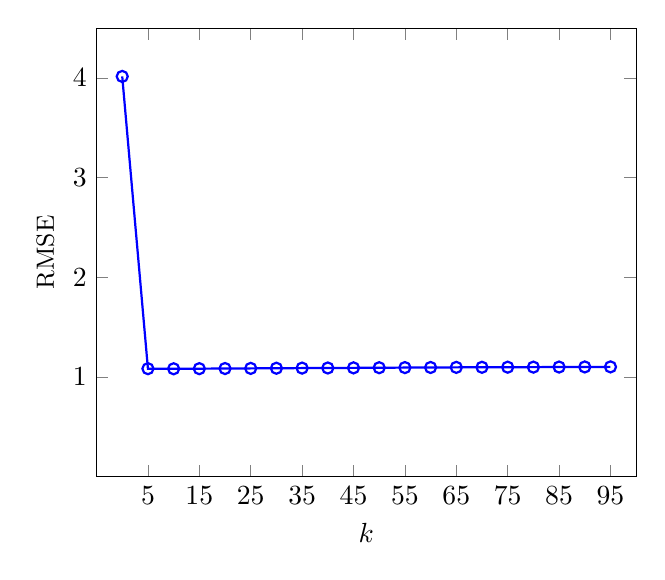
\begin{tikzpicture}
	\begin{axis}[
	xlabel={$k$},
	ylabel={\small{RMSE}},
	xmin=-5, xmax=100,
	ymin=0, ymax=4.5,
	xtick={5,15,25,35,45,55,65,75,85,95},
	ytick={1,2,3,4},
	x tick label style={color=black},
	legend style={
		draw=black,
		fill=white, 
		legend pos= north east,
		cells={anchor=west},},
	]
	\addplot[
		color=blue,
		mark=o,
		thick] 
		coordinates {(0,4.016120664688759)(5,1.0825649908614905)( 10,1.0815540472050764)(15,1.082655476468529)(20,1.084039420552301)(25, 1.08544809077967)(30,1.0870430839468697)(35,1.0883525165436614)(40,1.0894315213881094)(45,1.0906340685662301)(50,1.092158368755972)(55,1.0934254934023788)(60,1.0946167799674307)(65,1.0957557542153566)(70,1.096642058025502)(75,1.0975006311104656)(80,1.0980612147506275)(85,1.0989472280119372)(90,1.099854525492459)(95,1.1005504083912052)};
	\end{axis}
\end{tikzpicture}
\caption{RMSE in SVD with different $k$}
\label{fig:rmse}
\end{figure}

\begin{figure}[tbp]
\centering
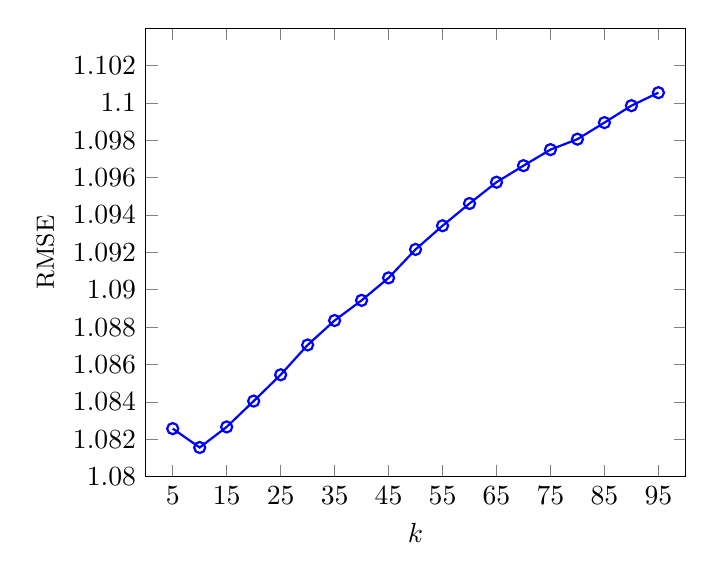
\begin{tikzpicture}
	\begin{axis}[
	xlabel={$k$},
	ylabel={\small{RMSE}},
	xmin=0, xmax=100,
	ymin=1.08, ymax=1.104,
	xtick={5,15,25,35,45,55,65,75,85,95},
	ytick={1.08,1.082,1.084,1.086,1.088,1.090,1.092,1.094,1.096,1.098,1.1,1.102},
	yticklabel style={/pgf/number format/.cd,fixed,precision=3},
	legend style={
		draw=black,
		fill=white, 
		legend pos= north east,
		cells={anchor=west},},
	]
	\addplot[
		color=blue,
		mark=o,
		thick] 
		coordinates {(5,1.0825649908614905)( 10,1.0815540472050764)(15,1.082655476468529)(20,1.084039420552301)(25, 1.08544809077967)(30,1.0870430839468697)(35,1.0883525165436614)(40,1.0894315213881094)(45,1.0906340685662301)(50,1.092158368755972)(55,1.0934254934023788)(60,1.0946167799674307)(65,1.0957557542153566)(70,1.096642058025502)(75,1.0975006311104656)(80,1.0980612147506275)(85,1.0989472280119372)(90,1.099854525492459)(95,1.1005504083912052)};
	\end{axis}
\end{tikzpicture}
\caption{RMSE in SVD with different $k$, shown in more detail}
\label{fig:rmse_detail}
\end{figure}

The second solution we are presenting here for comparison is a neural network. We trained a bidirectional LSTM. It has a bias layer, so that we could take into account that different people are rating higher or lower in general. We tried different dropout values, number of nodes, batch-sizes and trained over various epochs. In \rfig{lstm} you can see the Mean-Squared-Error loss over ten epochs of the neural network. We set a dropout of 0.75, 40 nodes in each layer and a batch size of 50, as these values were performing the best in our experiment. The best result we achieved on kaggle this way was an error of 1.04627. There are people that achieved much better results with a neural network \cite{tseng}, but our feeling is that our data was too sparse for this.

\begin{figure}[tbp]
\centering
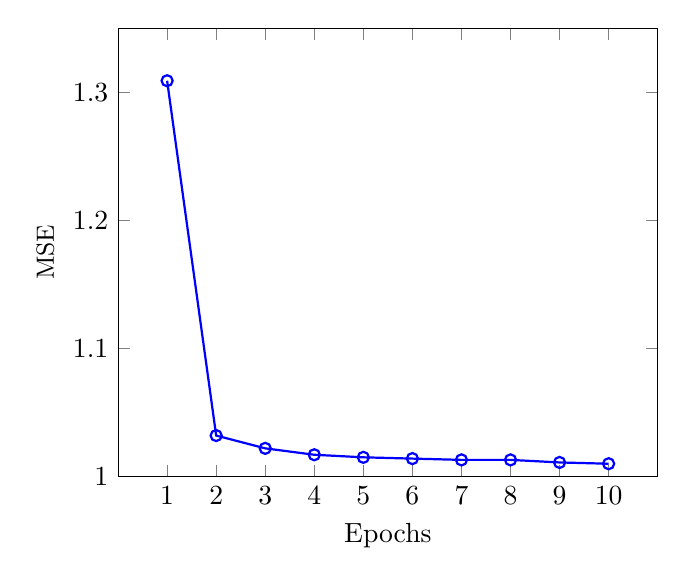
\begin{tikzpicture}
	\begin{axis}[
	xlabel={Epochs},
	ylabel={\small{MSE}},
	xmin=0, xmax=11,
	ymin=1.00, ymax=1.35,
	xtick={1,2,3,4,5,6,7,8,9,10},
	ytick={1.0,1.1,1.2,1.3},
	yticklabel style={/pgf/number format/.cd,fixed,precision=3},
	legend style={
		draw=black,
		fill=white, 
		legend pos= north east,
		cells={anchor=west},},
	]
	\addplot[
		color=blue,
		mark=o,
		thick] 
		coordinates {(1,1.309)(2,1.032)(3,1.022)(4,1.017)(5,1.015)(6,1.014)(7,1.013)(8,1.013)(9,1.011)(10,1.010)};
	\end{axis}
\end{tikzpicture}
\caption{MSE loss in LSTM over 10 epochs.}
\label{fig:lstm}
\end{figure}

Comparing the two solutions with our novel approach result of 0.98362 we can see that we managed to get much better results with.

\section{Summary}
In summary, our novel solution adopts ensemble learning approach and averages the results of different prediction algorithms, namely SVD, KNN-User-User-Pearson and KNN-Item-Item-Pearson. Traditional ensemble learning approaches usually train multiple models of a single learning algorithm. Here, our novel fusion approach managed to generate better results by first choosing the best parameters for the base collaborative filtering algorithms, then combining models with different algorithms as well as different parameters of the same algorithm as in a traditional approach. Experimental results suggest consistent better performance when several different algorithms are used. The final ensemble is then selected based on  cross-validation results in a systematic comparison of different algorithm combinations. 
This approach is also flexible and time-efficient in the case that more base CF algorithms are to be added and cross-validation needs to be carried out for a new ensemble. 
Since our solution computes a simple average of selected models, investigation into the performance of a weighted sum and how to obtain the optimal weights in the final ensemble might be required to achieve further improvement to the prediction results.

\nocite{*}
\bibliographystyle{IEEEtran}
\bibliography{report}
\end{document}
